% =====================================================================
%  Physics-Informed Neural Architectures for Double-Heston Option
%  Pricing: A Controlled Study
%
%  Rebuilt around the dh_pinn_v5 study (gated A5 architecture, market
%  ceiling, market-residual hybrid). Title retained from the earlier
%  v6 manuscript. Sections I-II reuse the earlier manuscript's prose.
%
%  Every number is traceable to a committed artifact; see
%  DATA_PROVENANCE.md. NOT compiled locally (no TeX toolchain here).
% =====================================================================
\documentclass[conference]{IEEEtran}
\IEEEoverridecommandlockouts

\usepackage{graphicx}
\usepackage{booktabs}
\usepackage{amsmath}
\usepackage{amssymb}
\usepackage{url}
\usepackage[hidelinks]{hyperref}
% Both are standard, but guard them so a missing .sty can never abort the build.
\IfFileExists{stfloats.sty}{\usepackage{stfloats}}{}
\IfFileExists{placeins.sty}{\usepackage{placeins}}{\providecommand{\FloatBarrier}{}}

% Float placement. The defaults strand large floats on near-empty pages;
% these values let more floats sit on a text page and raise the fill
% threshold a float page must meet before LaTeX will create one.
\renewcommand{\topfraction}{0.92}
\renewcommand{\bottomfraction}{0.70}
\renewcommand{\textfraction}{0.06}
\renewcommand{\floatpagefraction}{0.78}
\renewcommand{\dblfloatpagefraction}{0.78}
\setcounter{topnumber}{3}
\setcounter{bottomnumber}{2}
\setcounter{totalnumber}{5}
\setcounter{dbltopnumber}{3}

\graphicspath{{figures/}}

\begin{document}

\title{Physics-Informed Neural Architectures for\\
Double-Heston Option Pricing: A Controlled Study}

\author{\IEEEauthorblockN{Anonymous Submission}}

\maketitle

\begin{abstract}
Repeated Double-Heston valuation motivates fast neural surrogates, but
architecture gains are vulnerable to test-set selection and to being reported
without the trade-offs that accompany them. We conduct a frozen, staged
architecture study of a physics-informed pricing network for the two-factor
Heston model. A six-stage ablation at an identical budget isolates the
contribution of residual connections, layer-wise adaptive activations,
gradient-norm loss balancing, residual-adaptive collocation, and a gated
block. The winner was selected on development data alone and evaluated once on
an untouched 16,384-point exact-Double-Heston panel, where it is a
$1.61\times$ more accurate surrogate than the locked baseline (price RMSE
$1.062\times10^{-5}$ to $6.610\times10^{-6}$) at $4.7\%$ more parameters,
$1.7\times$ slower inference, and a $1.8\times$ worse PDE residual. We then
show that this fidelity gain is not the binding constraint in a real market:
on 10,706 S\&P~500 quotes the same improvement moves pricing error by $0.003$
volatility points out of $5.85$, because network error is about $1.3\%$ of
model misspecification. A small bounded residual head cuts held-out market
error by roughly two thirds, to $1.990$ volatility points, but under an
identical head the Double-Heston prior beats Black--Scholes ($p=0.018$) and
does \emph{not} beat the Single-Heston prior ($1.990$ against $1.917$,
$p=0.34$). Surrogate fidelity, physics consistency, market accuracy, and
compute remain competing criteria, and improving the first does not deliver
the second.
\end{abstract}

\begin{IEEEkeywords}
physics-informed neural networks, Double Heston, option pricing, scientific
machine learning, surrogate modeling
\end{IEEEkeywords}

% =====================================================================
\section{Introduction}

Repeated option valuation under stochastic volatility is expensive in
calibration, risk, and scenario workflows. Classical analytical formulas remain
indispensable baselines \cite{black1973,black1976}, while Heston's affine
stochastic-volatility model introduces a characteristic-function solution and a
nontrivial pricing PDE \cite{heston1993}. A two-factor extension can represent
distinct variance time scales and richer smile dynamics \cite{cjh2009}, but it
enlarges the state and parameter domains that a reusable pricing surrogate must
resolve.

Physics-informed neural networks (PINNs) combine labeled solutions with
differential-equation residuals evaluated by automatic differentiation
\cite{raissi2019,karniadakis2021}. Their flexibility does not remove
experimental hazards: composite losses can be poorly balanced
\cite{wang2021,wang2022}, optimization can fail even on apparently simple PDEs
\cite{krishnapriyan2021}, architecture choices can be tuned to an exposed test
set, and a favorable aggregate metric can conceal local regressions.

This paper asks two questions in sequence. First, under a controlled,
leakage-resistant protocol, which architectural ingredients actually improve
Double-Heston pricing fidelity? Second, and less often asked, what does a more
faithful surrogate buy when the model it approximates is itself confronted with
market data? The contributions are:

\begin{itemize}
\item a six-stage architecture ablation at an identical optimization budget,
      separating residual connections, adaptive activations, gradient-norm loss
      balancing, residual-adaptive collocation, and a gated block;
\item a winner selected on development data alone and evaluated once on an
      untouched 16,384-point exact-Double-Heston panel, giving a $1.61\times$
      fidelity improvement with its costs stated;
\item a quantified market ceiling showing that this improvement changes real
      S\&P~500 pricing error by $0.003$ of $5.85$ volatility points; and
\item an equal-capacity hybrid comparison in which the Double-Heston prior
      beats Black--Scholes but does not beat Single Heston, reported as a
      negative result.
\end{itemize}

The study concerns forward pricing surrogates. It does not claim unique
parameter recovery, trading profitability, or market-model superiority.

% =====================================================================
\section{Background and Related Work}

Black--Scholes and Black--76 give constant-volatility formulas for spot and
forward settings \cite{black1973,black1976}. Heston replaces constant variance
by a correlated square-root process \cite{heston1993}; multifactor variants can
represent distinct persistence and correlation effects in index-option smiles
\cite{cjh2009}. Characteristic-function pricing is commonly accelerated through
FFT or cosine expansions \cite{carr1999,fang2008}; stable complex-log handling
and efficient calibration remain material numerical issues
\cite{lord2010,cui2017}. These works motivate the high-accuracy Fourier
reference used here, rather than a learned model serving as its own target.

Neural differential-equation solvers predate modern PINNs \cite{lagaris1998},
while deep Galerkin and probabilistic approaches broadened high-dimensional PDE
computation \cite{sirignano2018,han2018}. PINNs and the wider physics-informed
learning framework impose governing equations through differentiable objectives
\cite{raissi2019,karniadakis2021,cuomo2022}. Such objectives can exhibit
optimization failure, gradient imbalance, and unequal convergence rates
\cite{wang2021,wang2022,krishnapriyan2021}. The modified MLP and the
gradient-norm annealing scheme of Wang, Teng, and Perdikaris are prior
methodology, not inventions of this study \cite{wang2021}; the same holds for
layer-wise adaptive activations \cite{jagtap2020}, training guidance
\cite{wang2023}, and residual-adaptive sampling \cite{wu2023}. Our ablation
isolates their individual contributions in a pricing setting.

Learning networks have long been studied for derivative pricing and hedging
\cite{hutchinson1994,ruf2020}. More recent parametric-PDE methods amortize
option valuation across model inputs \cite{glau2022}. Directly relevant
physics-informed work treats single-factor Heston pricing and option-pricing or
local-volatility PDEs \cite{hainaut2024,bae2024}; deep differential networks
have also been used for Heston calibration \cite{zhang2025}.

% =====================================================================
\section{Double-Heston PINN Formulation}

\subsection{Dynamics and Pricing PDE}

Under deterministic carry, let the asset return receive two independent factor
shocks,
\begin{align}
\frac{dS_t}{S_t} &= (r-q)\,dt + \sum_{i=1}^{2}\sqrt{v_{i,t}}\,dW^{S}_{i,t},\\
dv_{i,t} &= \kappa_i(\theta_i - v_{i,t})\,dt + \sigma_i\sqrt{v_{i,t}}\,dW^{v}_{i,t},
\end{align}
where $d\langle W^{S}_i, W^{v}_i\rangle_t = \rho_i\,dt$ and cross-factor shocks
are independent. With time to maturity $\tau$, log-forward moneyness
$x=\log(F/K)$, and strike-discount-normalized call $c = C/(Ke^{-r\tau})$, the
implemented PDE is
\begin{align}
0 = \;& c_\tau - \tfrac{1}{2}(v_1+v_2)\left(c_{xx}-c_x\right) \nonumber\\
 &- \sum_{i=1}^{2}\left[\kappa_i(\theta_i-v_i)c_{v_i}
   + \tfrac{1}{2}\sigma_i^2 v_i c_{v_i v_i}
   + \rho_i \sigma_i v_i c_{x v_i}\right],
\end{align}
with $c(x,v,0)=\max(e^{x}-1,0)$. Reported price errors use the
forward-normalized target $\tilde{c}=C/(e^{-r\tau}F)=e^{-x}c$.

Reference calls come from the separable Double-Heston characteristic function,
summing the two independent factor exponents and applying Gauss--Laguerre
Fourier inversion \cite{heston1993,carr1999,lord2010}. A 128-node result is
checked against a 96-node result; disagreement above $10^{-8}$ or a price-bound
breach triggers independent adaptive quadrature rather than clipping.

\subsection{Network, Prior, and Loss}

The network takes twelve inputs: the coordinates $x$, $v_1$, $v_2$, $\tau$ and,
per variance factor, $\kappa_i,\theta_i,\sigma_i,\rho_i$. These are expanded
into twenty-four engineered features, none of them learned, comprising four
general features, nine per factor, and two cross-factor terms. The output is a
bounded correction $1.8\tanh(\cdot)$ that enters the exponent of an analytic
baseline volatility $\sqrt{\bar v}$, giving implied volatility
$\sigma=\sqrt{\bar v}\,\exp\!\left(1.8\tanh(\cdot)\right)$, with
\begin{equation}
\bar v = \sum_{i=1}^{2}\left[\theta_i + (v_i-\theta_i)\frac{1-e^{-\kappa_i\tau}}{\kappa_i\tau}\right],
\end{equation}
after which a Black head converts implied volatility to price. The terminal
payoff is therefore exact by construction and price bounds cannot break.
Training combines normalized price and implied-volatility errors, the scaled
PDE residual, and a convexity penalty:
\begin{equation}
\mathcal{L} = \frac{\mathcal{L}_{p}}{(2\times10^{-5})^{2}}
 + \frac{\mathcal{L}_{\mathrm{IV}}}{0.002^{2}}
 + 0.1\,\frac{\mathcal{L}_{\mathrm{PDE}}}{0.01^{2}}
 + 0.1\,\mathcal{L}_{\mathrm{conv}} .
\end{equation}

The locked baseline is a width-256, five-layer plain $\tanh$ body with
$269{,}825$ float64 parameters, trained on 100,000 exact Fourier prices and
18,000 collocation points. The selected architecture replaces that body with a
gated block: shared encoders $U$ and $V$, and per level
\begin{align}
Z_\ell &= \tanh\!\left(a_\ell\,\mathrm{Linear}(h_{\ell-1})\right),\\
h_\ell &= (1-Z_\ell)\odot U + Z_\ell \odot V,
\end{align}
with five levels at width 256, giving $282{,}632$ parameters. The
prior-plus-correction design is preserved throughout; only the body and the
training mechanics change.

\begin{figure*}[!t]
\centering
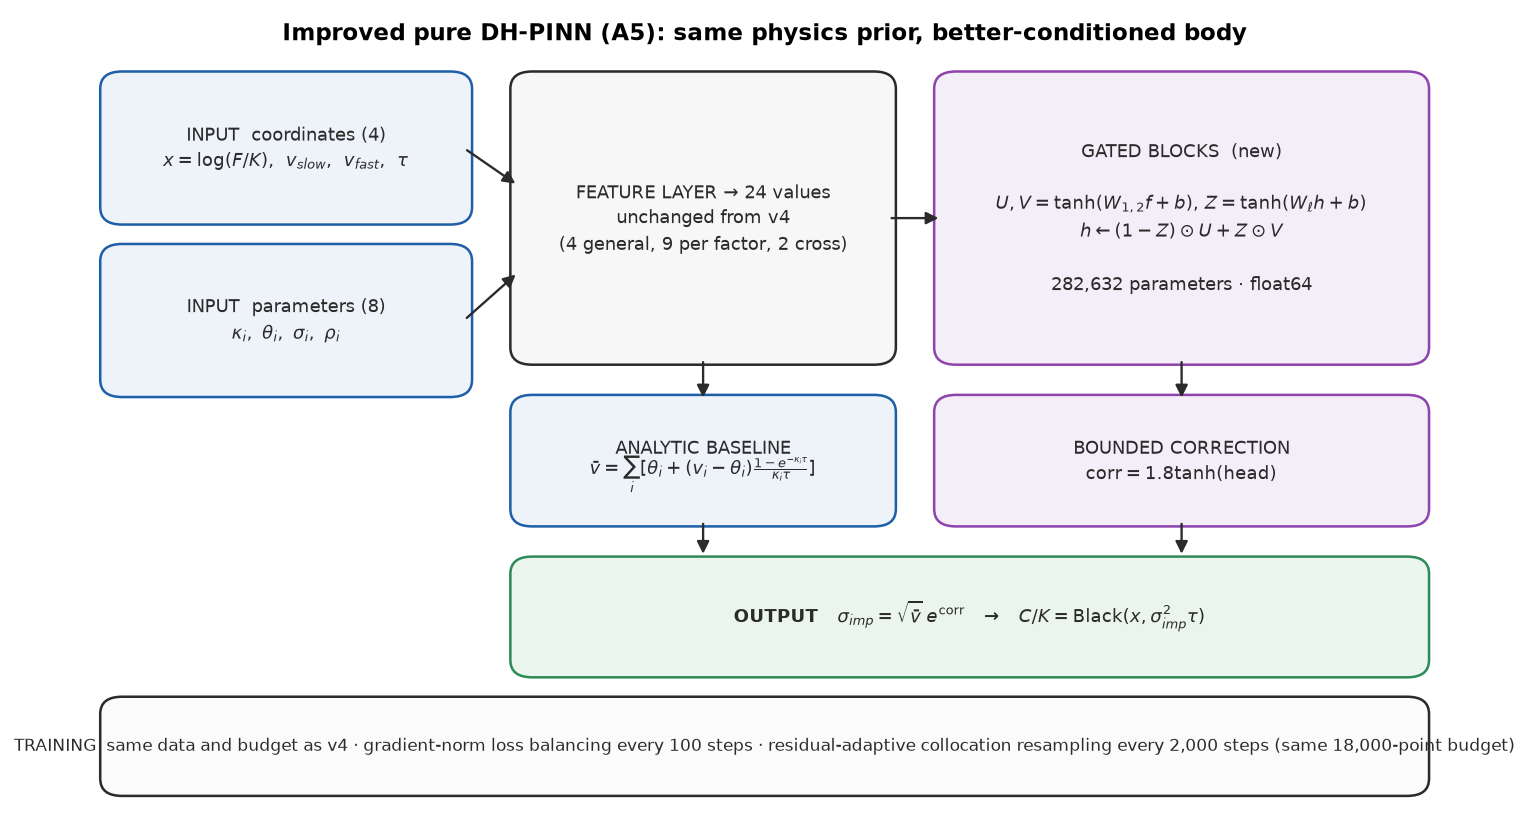
\includegraphics[width=\textwidth]{fig3_architecture.png}
\caption{Selected architecture. Twenty-four engineered features feed a gated
block with shared $U$/$V$ encoders; a bounded correction multiplies the
analytic baseline volatility, which a Black head converts to price.}
\label{fig:arch}
\end{figure*}

\begin{table}[!t]
\centering
\caption{Frozen supervision and collocation domain, inherited unchanged from
the locked baseline. $U$ and $\log$-$U$ denote uniform and log-uniform
sampling.}
\label{tab:domain}
\begin{tabular}{ll}
\toprule
Quantity & Frozen distribution \\
\midrule
Moneyness    & $x \sim U[-0.36,\,0.36]$ \\
Maturity     & $\tau \sim \log\text{-}U[7/365,\,730/365]$ yr \\
Variance     & $v_1 \sim \log\text{-}U[0.00015,\,0.18]$ \\
             & $v_2 \sim \log\text{-}U[0.001,\,0.22]$ \\
Shared scale & $s \sim U[0.7,\,3.2]$ \\
Slow factor  & $\kappa_1=0.9491$, $\theta_1=0.0257s$, \\
             & $\sigma_1=0.0517\sqrt{s}$, $\rho_1=0.7009$ \\
Fast factor  & $\kappa_2=10.7526$, $\theta_2=0.0330s$, \\
             & $\sigma_2=0.3613\sqrt{s}$, $\rho_2=-0.8916$ \\
Rate/carry   & $r=q=0$ after forward and discount normalization \\
\bottomrule
\end{tabular}
\end{table}

% =====================================================================
\section{Ablation and Protocol}

Every stage receives an identical budget: seed 17 only, 12,000 Adam steps with
learning rate $10^{-3}$ cosine-decayed to $10^{-5}$, 512 label and 128 physics
points per step, then 300 strong-Wolfe L-BFGS steps on the same data. The
locked baseline recipe (40,000 steps, two seeds) is reported alongside but is
not the ablation budget, so stage rows are comparable only to one another.

The stages are cumulative. \textsc{a0} is the locked plain $\tanh$ stack
retrained at the ablation budget. \textsc{a1} adds residual blocks
$h \leftarrow h + \alpha_\ell\tanh(\mathrm{Linear}(h))$ with $\alpha_\ell$
learned per block. \textsc{a2} adds layer-wise adaptive activations
$\tanh(a_\ell z)$ \cite{jagtap2020}. \textsc{a3} adds gradient-norm loss
balancing \cite{wang2021}. \textsc{a4} adds residual-adaptive collocation
\cite{wu2023}. \textsc{a5} replaces the residual block with the gated block.

Four disjoint panels were drawn in advance: 8,192 development points (seed
93201) used only to choose the ablation winner and the hybrid
hyper-parameters; 16,384 final fidelity points (seed 93202) held untouched
until the architecture was frozen and opened once; 4,096 PDE points (seed
93203); and a 6,144-point short-maturity diagnostic (seed 93204) used for
reporting only, never for selection. The selection rule was fixed in advance:
lowest development price RMSE, with a simpler stage winning if within $5\%$.
\textsc{a5} won and was retrained at the full locked recipe with two seeds
before the final panel was opened. A stopping rule was also fixed in advance:
once implied-volatility RMSE against the exact model falls below $0.07$
volatility points, architecture work stops and the residual market error is
attributed, with numbers, to model misspecification.

% =====================================================================
\section{Results}

\subsection{Which Ingredients Matter}

Table~\ref{tab:ablation} gives the ablation. Residual connections are the
single largest effect, lowering price error $3.1\times$ against the plain stack
at the same budget and essentially the same parameter count. Adaptive
activations add a further $21\%$. Gradient-norm balancing improves
implied-volatility error from $0.158$ to $0.116$ but \emph{raises} price error,
because it reweights away from the price term by construction.
Residual-adaptive collocation mainly repairs the physics residual, from
$0.082$ to $0.036$, at no extra cost. The gated block wins on every metric for
$4.7\%$ more parameters.

\begin{table*}[!t]
\centering
\caption{Six-stage ablation at an identical budget (seed 17, 12,000 Adam steps,
300 L-BFGS), scored on the 8,192-point development panel that also drove
selection. Stages are cumulative. The locked baseline row uses a larger recipe
and is context, not a comparable row; its values here are not those of
Table~\ref{tab:fidelity}, which reports the untouched 16,384-point panel
($1.062\times10^{-5}$, $0.1175$).}
\label{tab:ablation}
\begin{tabular}{llrrr}
\toprule
Stage & Change & Params & Price RMSE & IV RMSE \\
\midrule
locked & 40k steps, 2 seeds & 269,825 & $1.081\times10^{-5}$ & 0.1125 \\
\midrule
\textsc{a0} & plain $\tanh$ stack & 269,830 & $6.144\times10^{-5}$ & 0.3513 \\
\textsc{a1} & + residual blocks & 269,834 & $1.985\times10^{-5}$ & 0.1904 \\
\textsc{a2} & + adaptive $\tanh$ & 269,834 & $1.572\times10^{-5}$ & 0.1575 \\
\textsc{a3} & + gradient balancing & 269,834 & $2.549\times10^{-5}$ & 0.1157 \\
\textsc{a4} & + adaptive collocation & 269,834 & $2.475\times10^{-5}$ & 0.1197 \\
\textsc{a5} & + gated block & 282,632 & $\mathbf{1.471\times10^{-5}}$ & $\mathbf{0.1051}$ \\
\bottomrule
\end{tabular}
\end{table*}

\begin{figure}[!t]
\centering
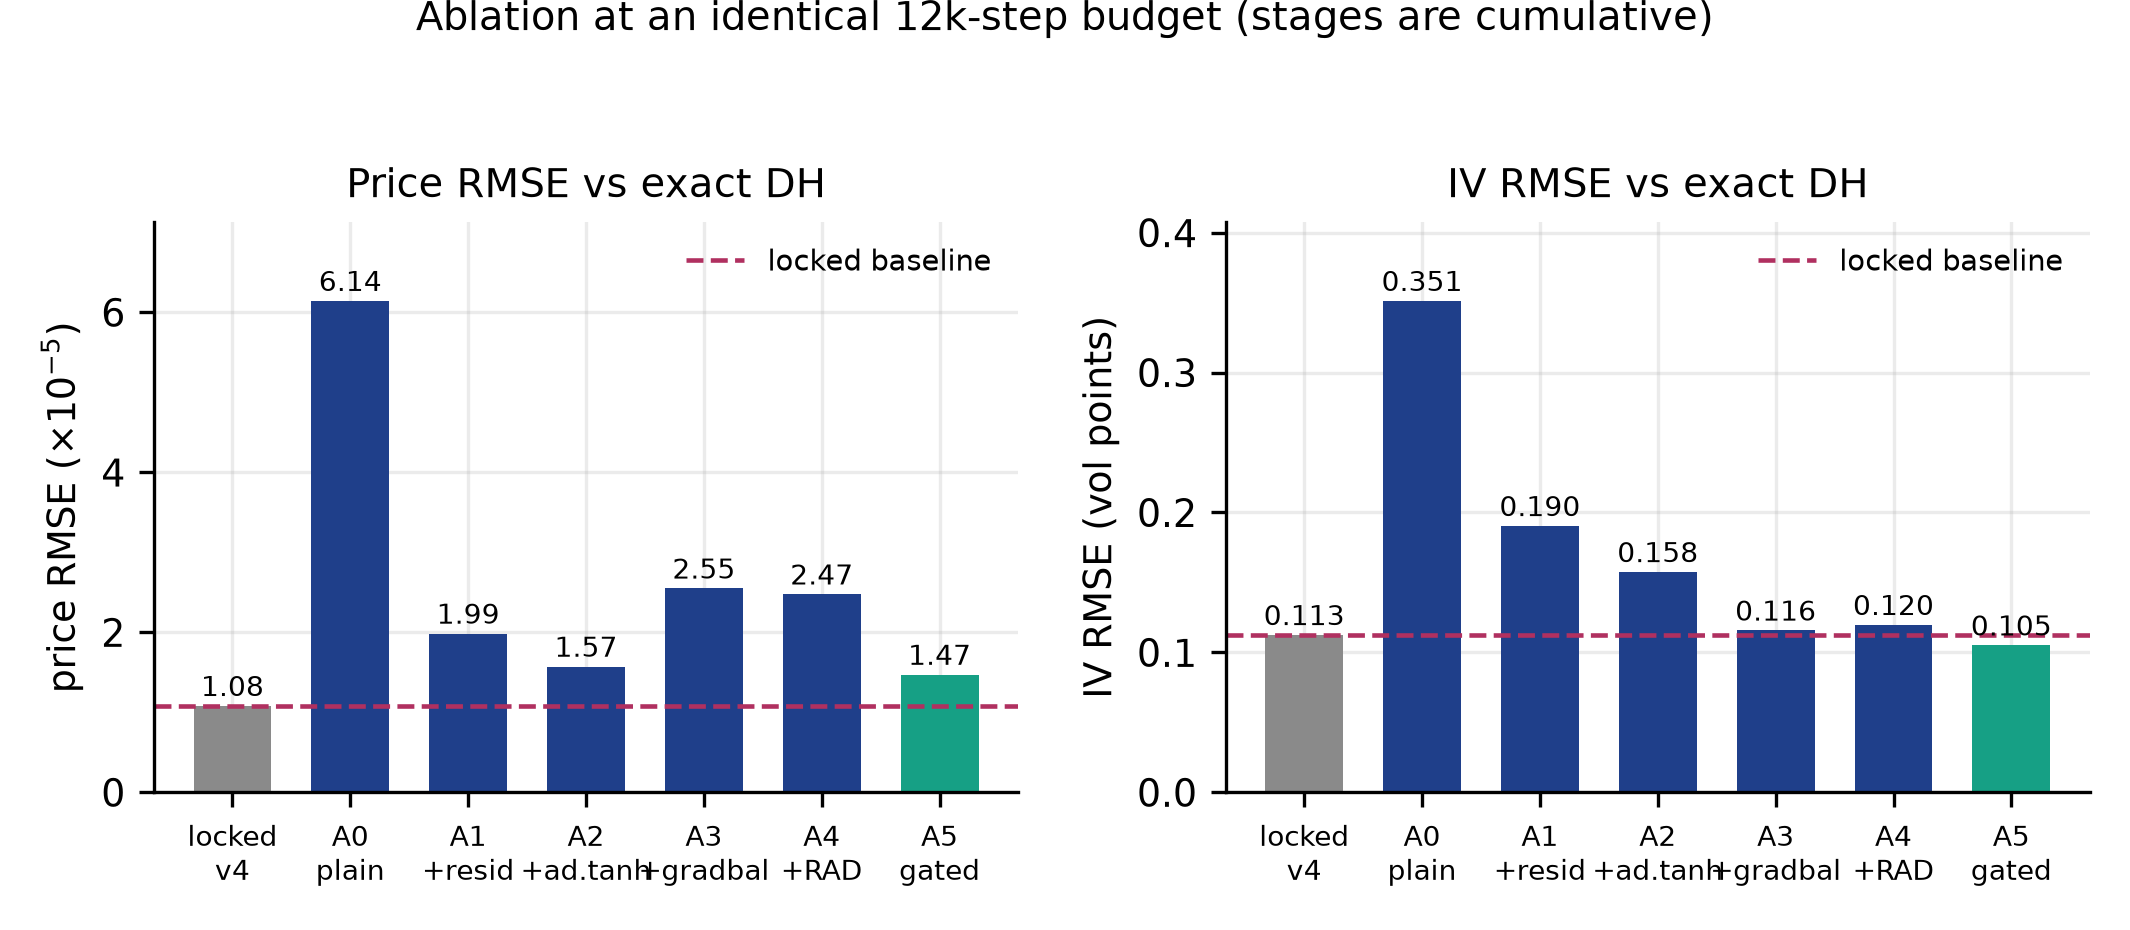
\includegraphics[width=\columnwidth]{fig1_ablation.png}
\caption{Ablation at an identical budget. Residual connections dominate;
gradient balancing trades price accuracy for implied-volatility accuracy.}
\label{fig:ablation}
\end{figure}

\subsection{Fidelity on the Untouched Panel}

Table~\ref{tab:fidelity} compares the locked baseline with the selected
architecture on the 16,384-point panel, opened once. Price RMSE improves
$1.61\times$, the worst case $2.56\times$, implied volatility $1.59\times$, and
short-maturity at-the-money error $1.95\times$. Against the predeclared
targets, price RMSE below $7\times10^{-6}$ was met; the implied-volatility
target of $0.07$ was just missed at $0.0738$; neither stretch target was met.

The costs are stated rather than omitted: $4.7\%$ more parameters,
$1.7\times$ slower inference per quote, and a PDE residual that is
$1.8\times$ \emph{worse}, because gradient balancing moved weight toward the
supervised terms. Appendix~\ref{app:curves} verifies that the surrogate
nevertheless remains a valid option price.

\begin{table*}[!t]
\centering
\caption{Exact-Double-Heston fidelity on the untouched 16,384-point panel,
opened once. Two seeds averaged.}
\label{tab:fidelity}
\begin{tabular}{lrrl}
\toprule
Metric & Locked & Selected & Ratio \\
\midrule
Price RMSE & $1.062\times10^{-5}$ & $\mathbf{6.610\times10^{-6}}$ & $1.61\times$ better \\
Price P95 & $2.258\times10^{-5}$ & $1.419\times10^{-5}$ & $1.59\times$ \\
Price max & $1.523\times10^{-4}$ & $5.938\times10^{-5}$ & $2.56\times$ \\
IV RMSE & $0.1175$ & $\mathbf{0.0738}$ & $1.59\times$ \\
7--30 d IV RMSE & $0.2232$ & $0.1429$ & $1.56\times$ \\
Short-ATM IV RMSE & $0.0618$ & $0.0317$ & $1.95\times$ \\
\midrule
PDE residual & $\mathbf{0.0309}$ & $0.0558$ & $1.8\times$ \emph{worse} \\
Parameters & 269,825 & 282,632 & $+4.7\%$ \\
Inference & 14.2 $\mu$s/quote & 24.8 $\mu$s/quote & $1.7\times$ slower \\
\bottomrule
\end{tabular}
\end{table*}

\begin{figure}[!t]
\centering
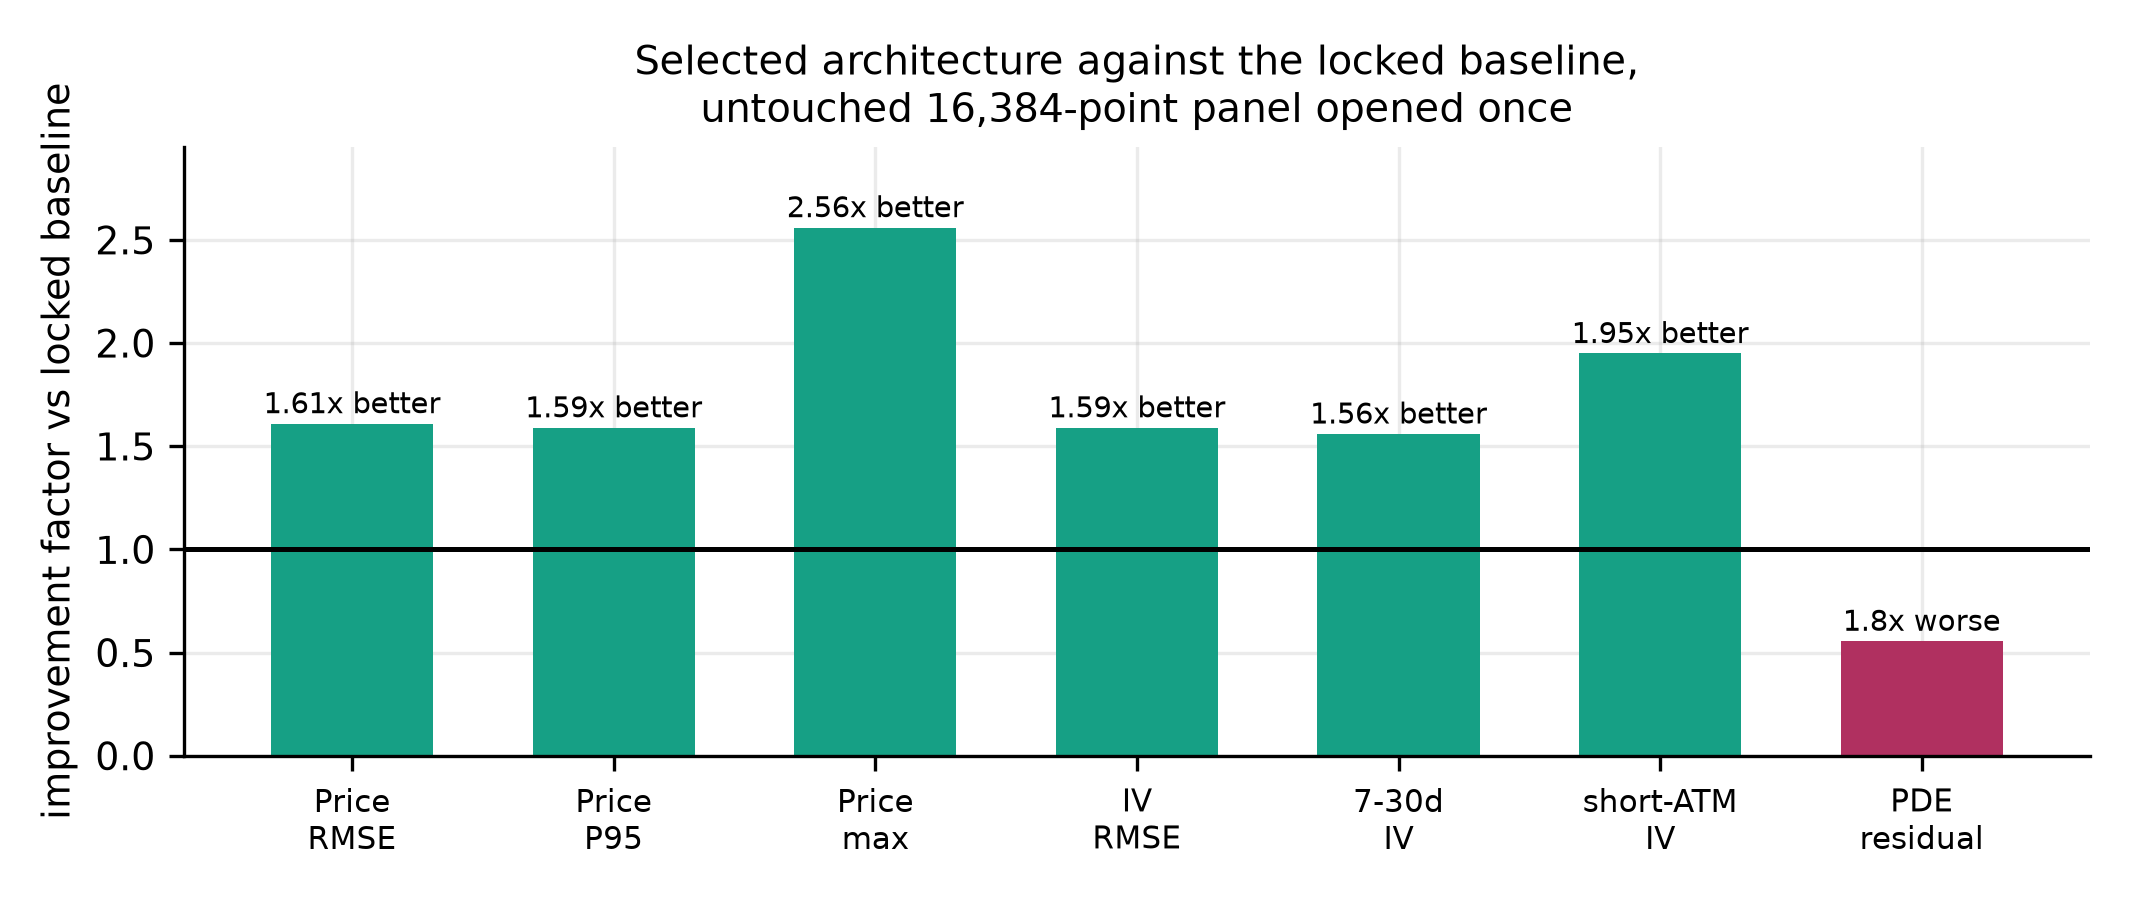
\includegraphics[width=\columnwidth]{fig2_old_vs_new.png}
\caption{Locked baseline against the selected architecture on the untouched
panel. The accuracy gain is real; the physics residual moves the other way.}
\label{fig:oldnew}
\end{figure}

\subsection{The Market Ceiling}

We then price 10,706 S\&P~500 index-option quotes with published
parameters, fitting at most a single level scale. These quotes are a single
trading-day snapshot (quote date 23 September 2026, VIX 14.2) covering 47
expiries, so the result is one cross-section rather than a time series; the
breadth check in Appendix~\ref{app:market} is what addresses other surfaces. Table~\ref{tab:spx} gives the
result. Exact Double Heston reaches $5.818$ volatility points with a level
scale fitted; the locked surrogate reaches $5.850$ and the improved surrogate
$5.847$.

The improved network reduced its distance to the exact model by $0.044$
volatility points, from $0.1175$ to $0.0738$. Its market error changed by
$0.003$. The network's error is about $1.3\%$ of the market gap, and a
\emph{perfect} surrogate would still sit at $5.818$. The entire remaining
$5.8$ is model and parameter misspecification. This is the central negative
finding of the study: architecture work cannot repair a fixed-parameter
model's market error.

\begin{table}[!t]
\centering
\caption{S\&P~500 benchmark, 10,706 quotes, VIX 14.2. IV RMSE in volatility
points. Structural parameters are published and never refitted.}
\label{tab:spx}
\begin{tabular}{lrr}
\toprule
Model & Nothing fitted & Level scale fitted \\
\midrule
Black--Scholes, fixed vol & 6.855 & 7.271 \\
Single Heston, published & 5.359 & 5.788 \\
Double Heston, published & $\mathbf{5.344}$ & 5.818 \\
Surrogate, locked & 5.365 & 5.850 \\
Surrogate, selected & 5.364 & 5.847 \\
\bottomrule
\end{tabular}
\end{table}

\begin{figure}[!t]
\centering
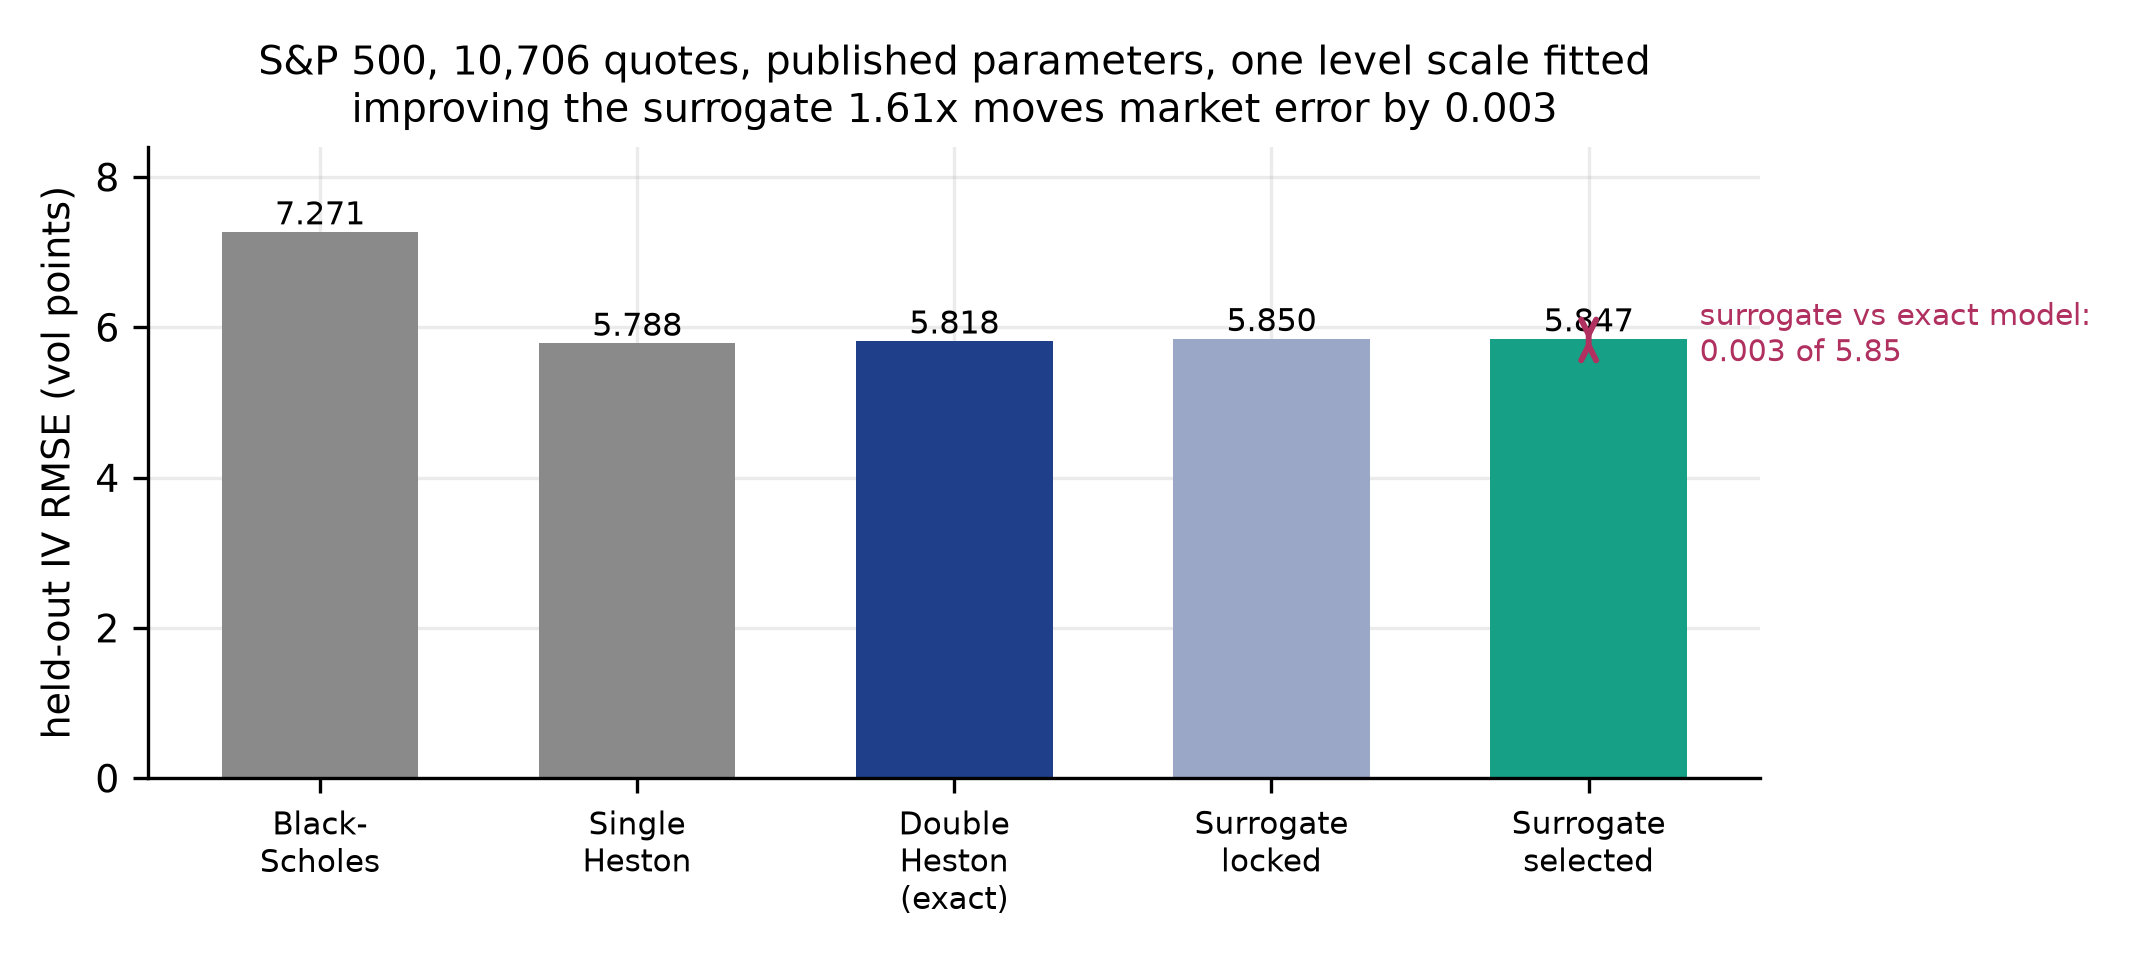
\includegraphics[width=\columnwidth]{fig4_market_benchmark.png}
\caption{Market benchmark. The surrogate tracks the exact model closely; both
sit far from the quotes, and the distance between them is negligible beside the
distance to the market.}
\label{fig:market}
\end{figure}

\subsection{An Equal-Capacity Hybrid, and a Negative Result}

The predeclared stopping rule did not strictly fire: implied-volatility RMSE
reached $0.0738$ against its $0.07$ threshold. We stopped architecture work
there regardless, because the ceiling quantified in Section~V-C does not depend
on the remaining $0.004$. We then test whether a small bounded correction
closes the market gap, and whether the two-factor prior helps once such a
correction is allowed. The surface is split by a frozen
checkerboard on (expiry rank, strike rank) into 4,271 calibration, 1,082
development, and 5,353 held-out quotes; held-out quotes are never inputs, never
train the head, and never select hyper-parameters.

The head is identical for every prior: inputs
$[x,\log\tau,\text{prior IV},x/\sqrt{\tau}]$ standardized on calibration
statistics, then $\mathrm{Linear}(4,64)\to\tanh\to\mathrm{Linear}(64,64)\to
\tanh\to\mathrm{Linear}(64,1)$, with
$\Delta\mathrm{IV}=\delta_{\max}\tanh(\cdot)$ added to the prior implied
volatility before the Black head. That is $4{,}545$ parameters. Structural
parameters never change.

The hybrid cuts held-out error by roughly two thirds
(Table~\ref{tab:hybrid}). But the gain comes from the head, not the prior. In a
like-for-like comparison over 19 maturity-by-moneyness cells
(Table~\ref{tab:prior}), the Double-Heston prior beats Black--Scholes
($+0.580$, 13/19 cells, $p=0.018$) and does \emph{not} beat Single Heston
($+0.020$, 9/19 cells, $p=0.34$). The desired ordering did not appear and has
not been manufactured. A residual-complexity diagnostic predicted this: after
the level fit, the residual left by Double Heston ($5.797$) is
indistinguishable from Single Heston's ($5.801$). It is smoother across
maturity ($0.678$ against $0.794$) but no smaller, so the same small head
learns it about equally well. We also note that $\delta_{\max}$ selected the
largest value on its grid for every prior, so the bound binds.

\begin{table*}[!t]
\centering
\caption{Market-residual hybrid, held-out S\&P~500 quotes. Every prior receives
an identical 4,545-parameter head. This is a hybrid, not exact Double Heston.}
\label{tab:hybrid}
\begin{tabular}{lrrr}
\toprule
Prior & Prior only & + head & Mean $|\Delta\mathrm{IV}|$ \\
\midrule
Black--Scholes & 7.274 & 2.366 & 4.33 \\
Single Heston & 5.773 & $\mathbf{1.917}$ & 3.33 \\
Double Heston, exact & 5.839 & 1.990 & 3.35 \\
Double Heston, surrogate & 5.850 & 1.970 & 3.36 \\
\bottomrule
\end{tabular}
\end{table*}

\begin{table}[!t]
\centering
\caption{Equal-capacity prior comparison over 19 held-out cells. Positive mean
difference favors Double Heston.}
\label{tab:prior}
\begin{tabular}{lrrrl}
\toprule
Comparison & Mean diff. & Cells & $p$ & DH wins? \\
\midrule
BS $-$ DH & $+0.580$ & 13/19 & 0.018 & \textbf{yes} \\
SH $-$ DH & $+0.020$ & 9/19 & 0.340 & \textbf{no} \\
\bottomrule
\end{tabular}
\end{table}

\begin{figure}[!t]
\centering
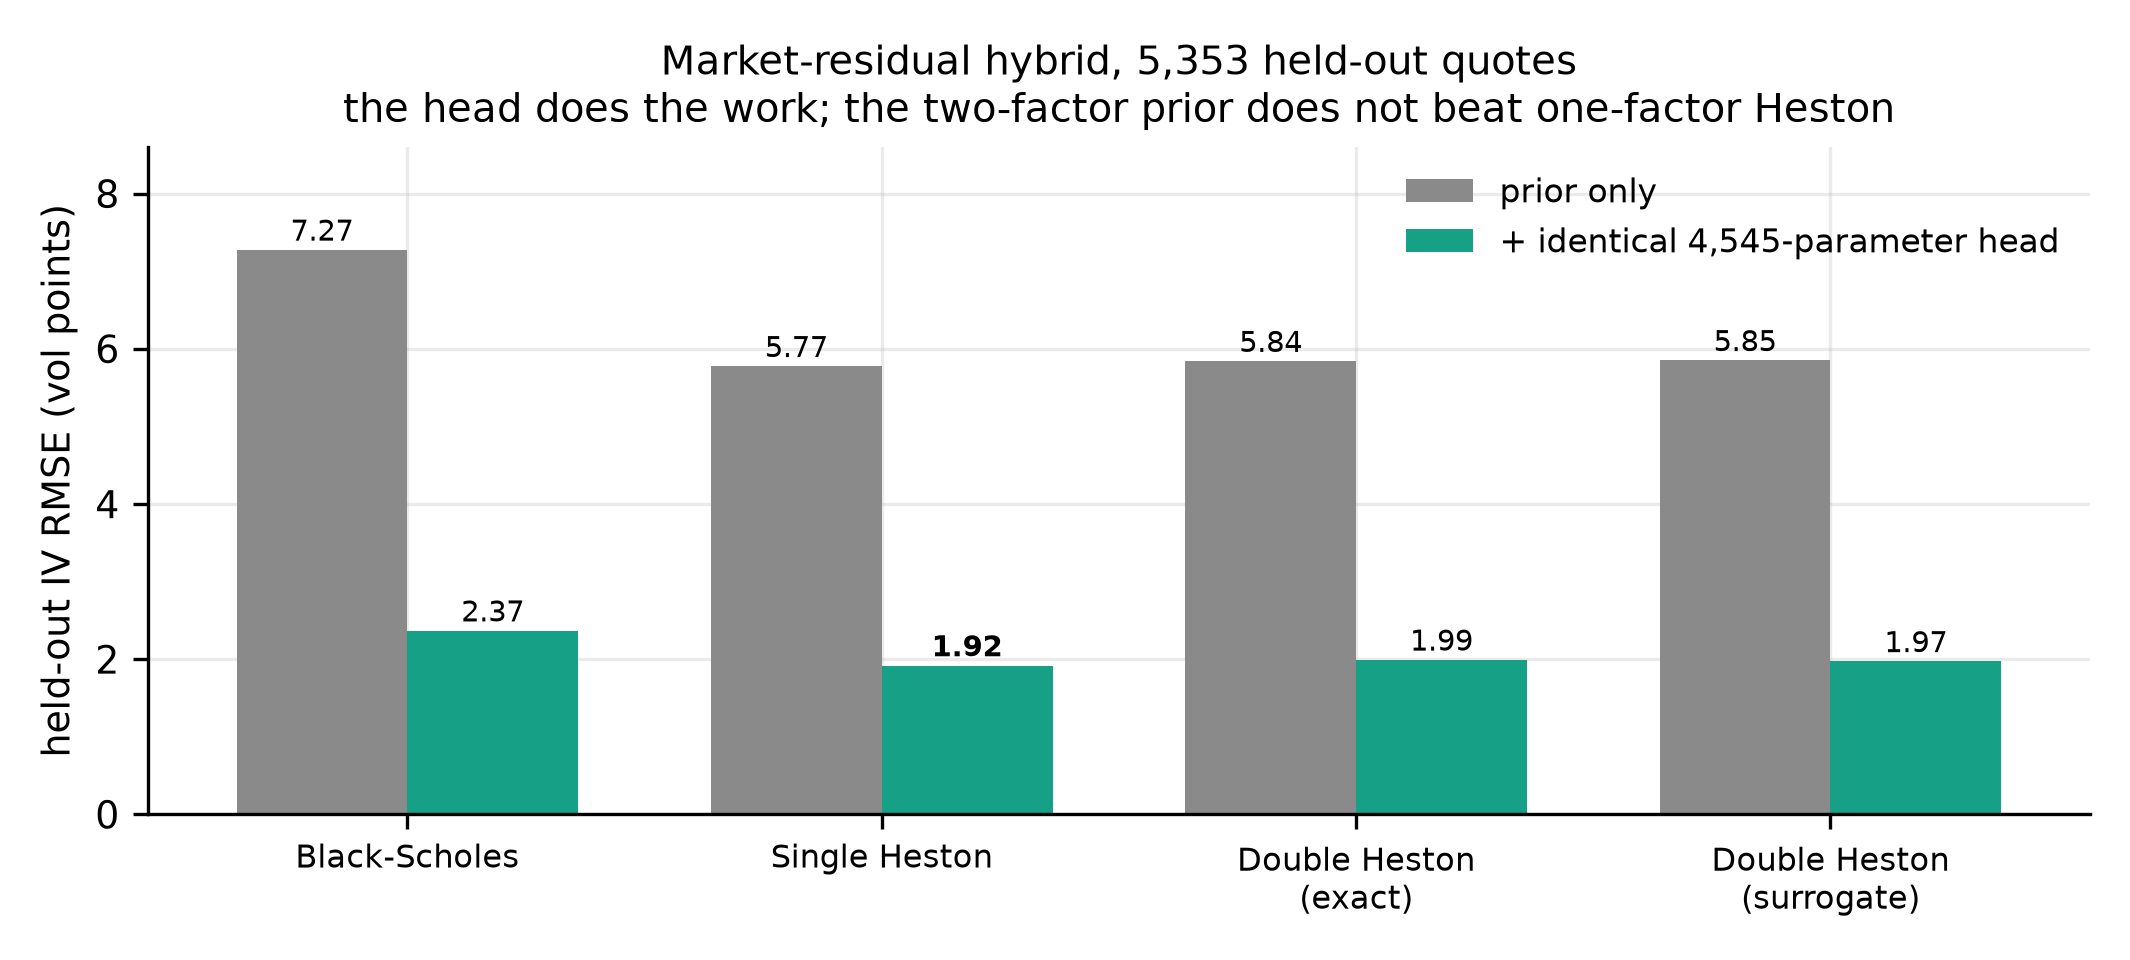
\includegraphics[width=\columnwidth]{fig5_track_b.png}
\caption{Market-residual hybrid. Held-out error falls by about two thirds for
every prior, and the ordering between priors is essentially unchanged: the
correction, not the prior, does the work.}
\label{fig:trackb}
\end{figure}

A no-arbitrage control on the held-out grid found no monotonicity violations
for any hybrid. Convexity violations number 773--866 of roughly 5,250 triples
and calendar violations roughly 660 of 5,330; the raw market quotes on the same
grid show 1,087 convexity violations, so the hybrids are smoother than the data
they fit rather than broken.

% =====================================================================
\section{Limitations}

The fidelity benchmark uses exact-Double-Heston synthetic targets and measures
approximation quality, not model validity. The ablation uses a single seed at a
shared budget, and only the winner was retrained with two seeds; two seeds
cannot characterize seed-level variability. The PDE residual worsens while
price accuracy improves, so the two objectives are in tension and we do not
claim joint improvement. The market study uses published structural parameters
and fits at most a level scale; per-date calibration, which the ordering in
Appendix~\ref{app:market} suggests is what actually moves market error, is not
performed here. The hybrid is explicitly a hybrid and must not be read as exact
Double Heston. Finally, parameter identifiability and inverse calibration are
separate problems and are not evaluated.

% =====================================================================
\section{Conclusion}

A controlled ablation identified residual connections as the dominant
architectural ingredient for a Double-Heston pricing PINN, with a gated block
selected on development data and confirmed once on an untouched panel at
$1.61\times$ the baseline fidelity. The improvement is genuine and its costs
are explicit: more parameters, slower inference, and a worse PDE residual.

The more consequential result is what that fidelity does not buy. On real
index options the improvement moves pricing error by $0.003$ of $5.85$
volatility points, because network error is roughly $1.3\%$ of model
misspecification. A small equal-capacity residual head closes two thirds of the
remaining gap, but it does so regardless of the prior: the two-factor prior
beats Black--Scholes and does not beat one-factor Heston. Future work should
target per-date structural calibration and richer priors for the steep
low-strike wing rather than additional network capacity, and should predeclare
an untouched market panel before any such claim is made.

% =====================================================================
\appendices

\section{Pricing-Curve Validation}
\label{app:curves}

Error metrics do not establish that a surrogate remains a valid option price.
This appendix reports that check on a controlled benchmark with $r=q=0$ and
$K=100$, so the forward equals the spot and the arbitrage bounds take their
simplest form. The variance state is a frozen two-timescale pair with
$v_{\text{fast}}+v_{\text{slow}}=0.04$, a $20\%$ instantaneous volatility, and
$\kappa$ values in the ratio $11.3$. Curves are evaluated on one shared
601-point grid in $S$ and a 601-point grid in $\tau$, and the network is drawn
only inside its trained domain $|\log(S/K)|\le0.36$.

Fig.~\ref{fig:appS} plots price against underlying price at six maturities for
the exact model and the network, with residuals beneath.
Fig.~\ref{fig:apptau} plots price against time to maturity at the money. Both
are prices, not implied volatilities. Following the usual convention, the
maturity axis \emph{decreases} left to right, so the horizontal direction is
time running forward toward expiry at the right edge and the curve decays to
its payoff. The underlying relation is the standard one,
$\partial C/\partial\tau\ge0$: an option with more time remaining is worth
more, which is the same statement as $\partial C/\partial t\le0$ because
$\tau=T-t$.

Across the 34 distinct model-by-maturity curves on this $r=q=0$ benchmark
there were no violations of $\partial C/\partial S\ge0$, of
$C\ge\max(S-K,0)$, or of $C\le S$. The underlying validation file also records
six curves from a separate Black--Scholes PINN under its own $r=0.03$,
$q=0.01$ convention; those are not part of this benchmark and are excluded
here. Convexity
held for every exact pricer and for the network, the worst value being of order
$10^{-9}$ and therefore at floating-point level. Monotonicity of price in
maturity was verified rather than imposed: all 20 distinct adjacent-maturity
comparisons among the exact pricers increased with $\tau$, and on the 600-step
$\tau$ grid each of the five curves, the network included, decays monotonically
toward expiry. Against the exact price the network's RMSE was
$2.7\times10^{-4}$ at 30 days and $1.4\times10^{-3}$ at 730 days in currency
units: $158\times$ and $716\times$ below the distance to a constant-volatility
baseline, and $148\times$ and $71\times$ below a one-factor Heston baseline.

\begin{figure}[!t]
\centering
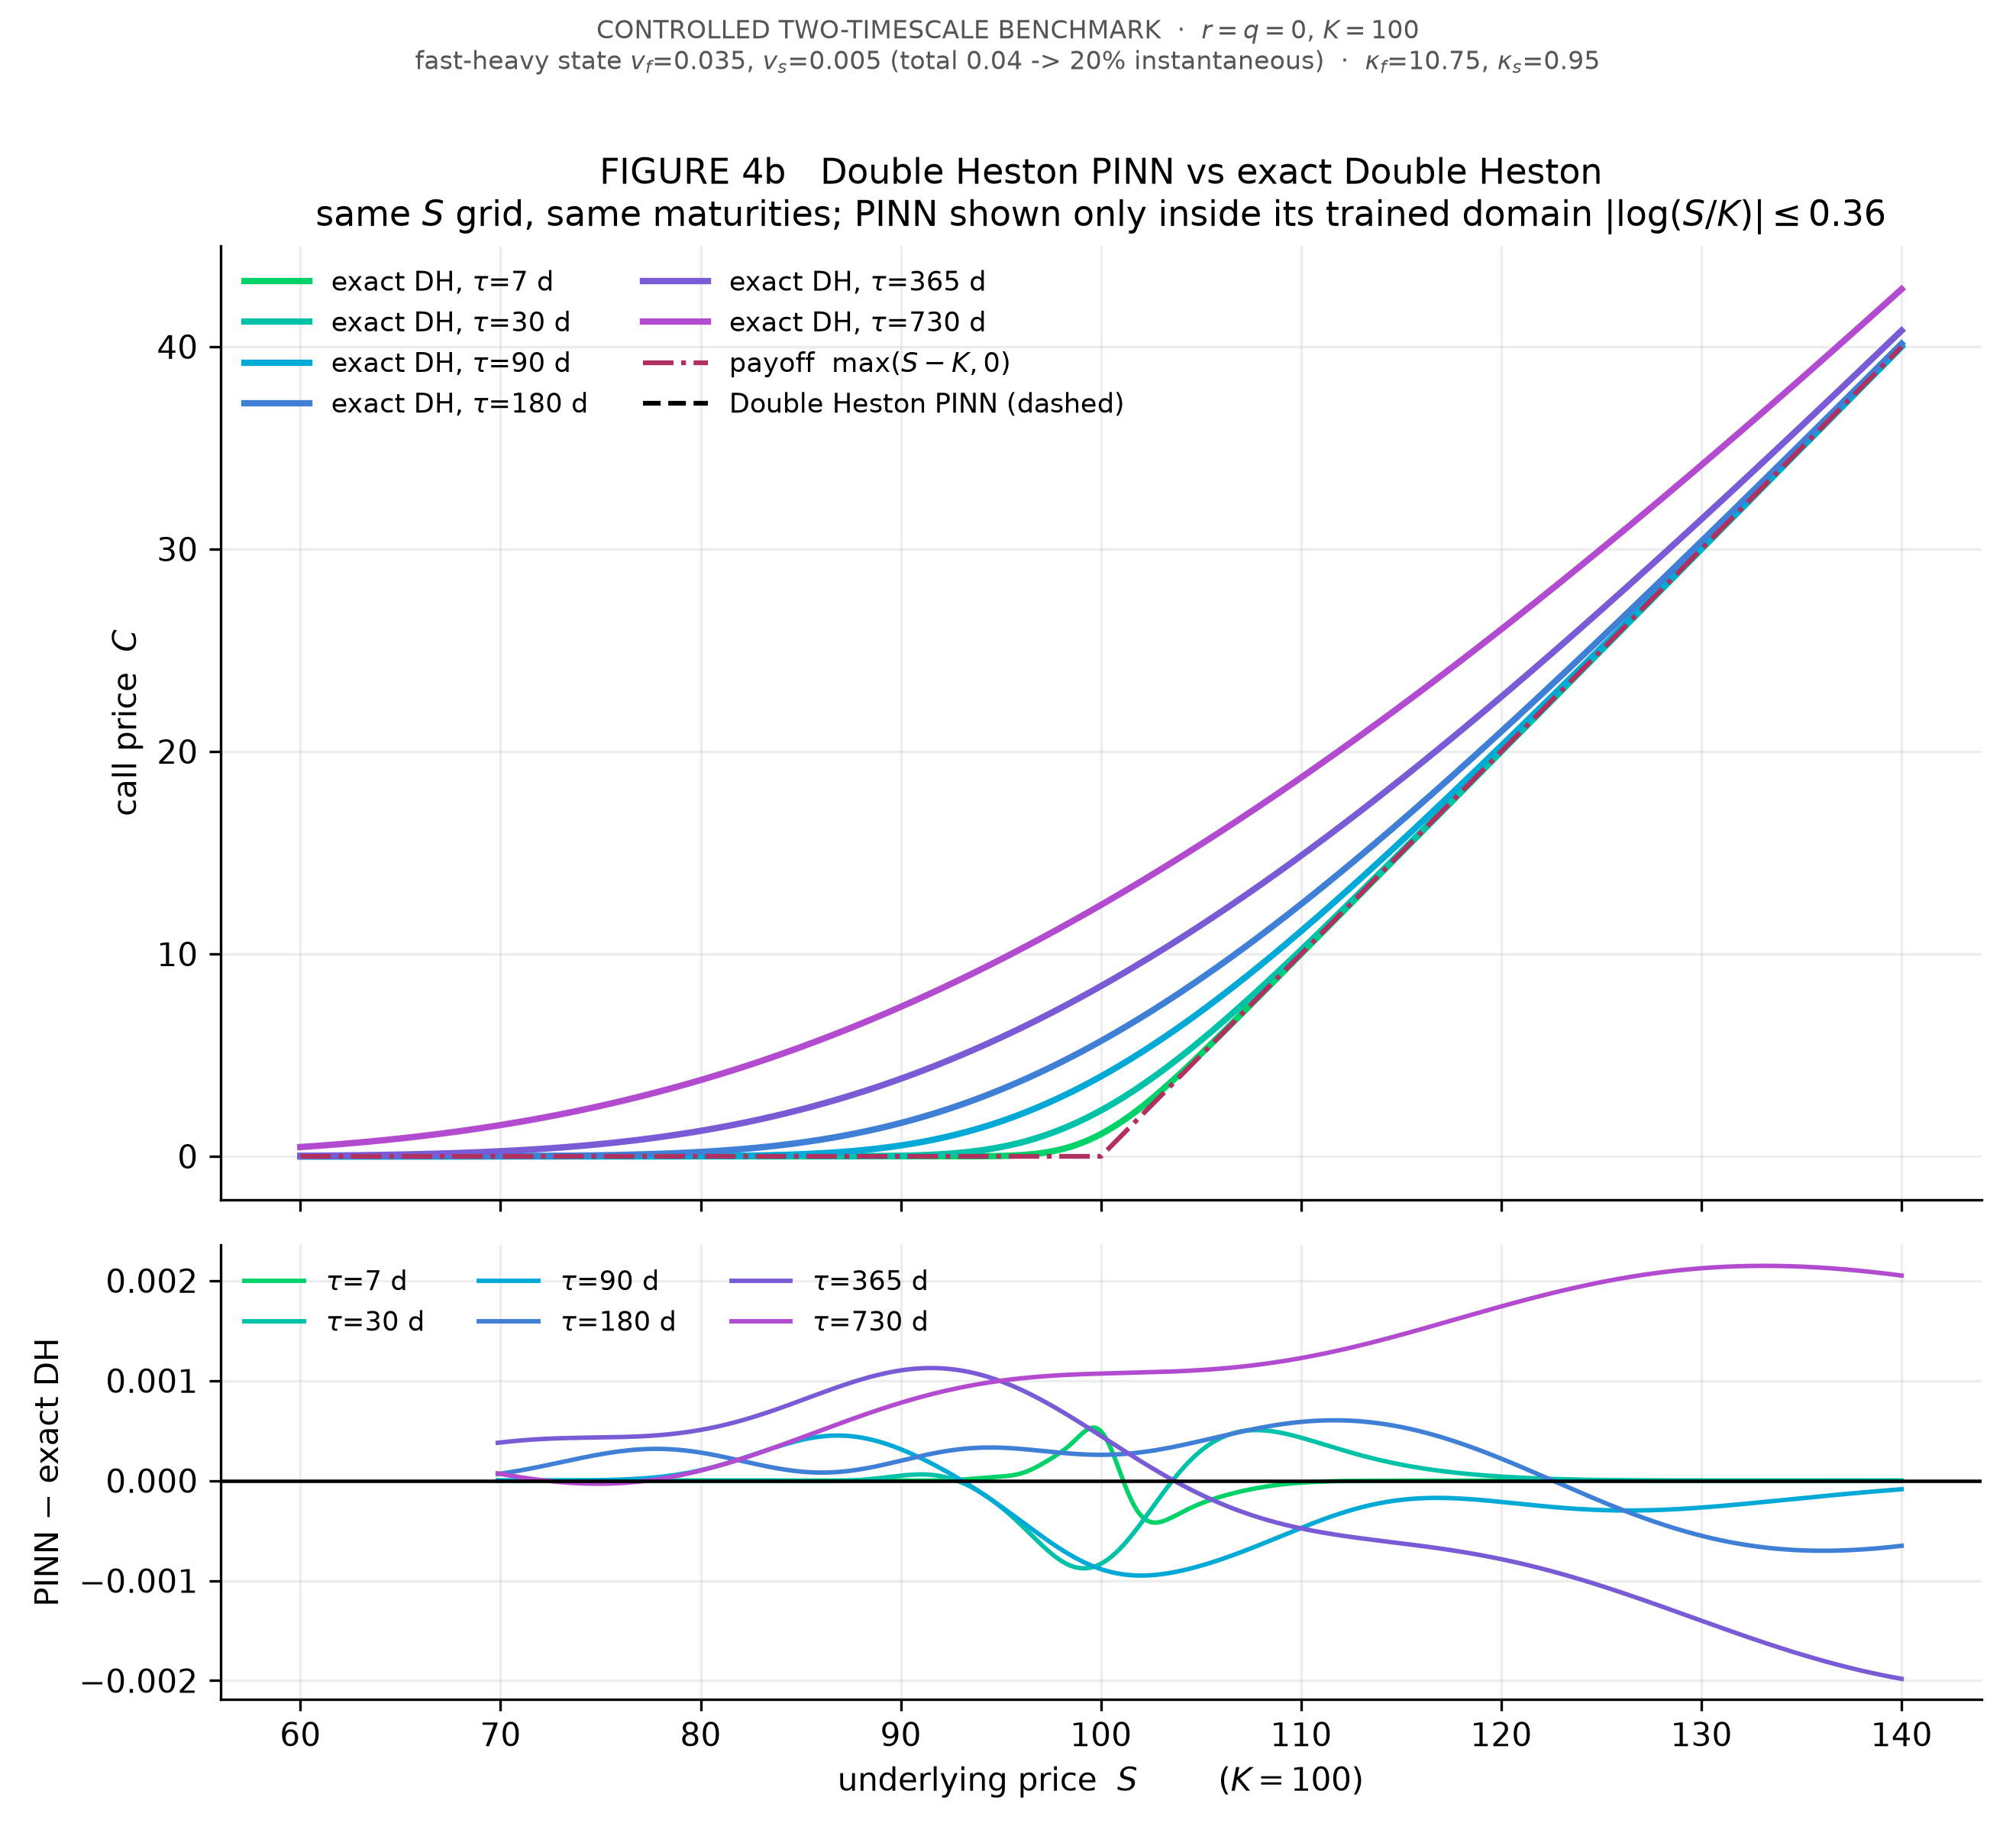
\includegraphics[width=\columnwidth]{figA1_C_vs_S.png}
\caption{Call price against underlying price at six maturities, exact model and
network, with residuals beneath.}
\label{fig:appS}
\end{figure}

\begin{figure}[!t]
\centering
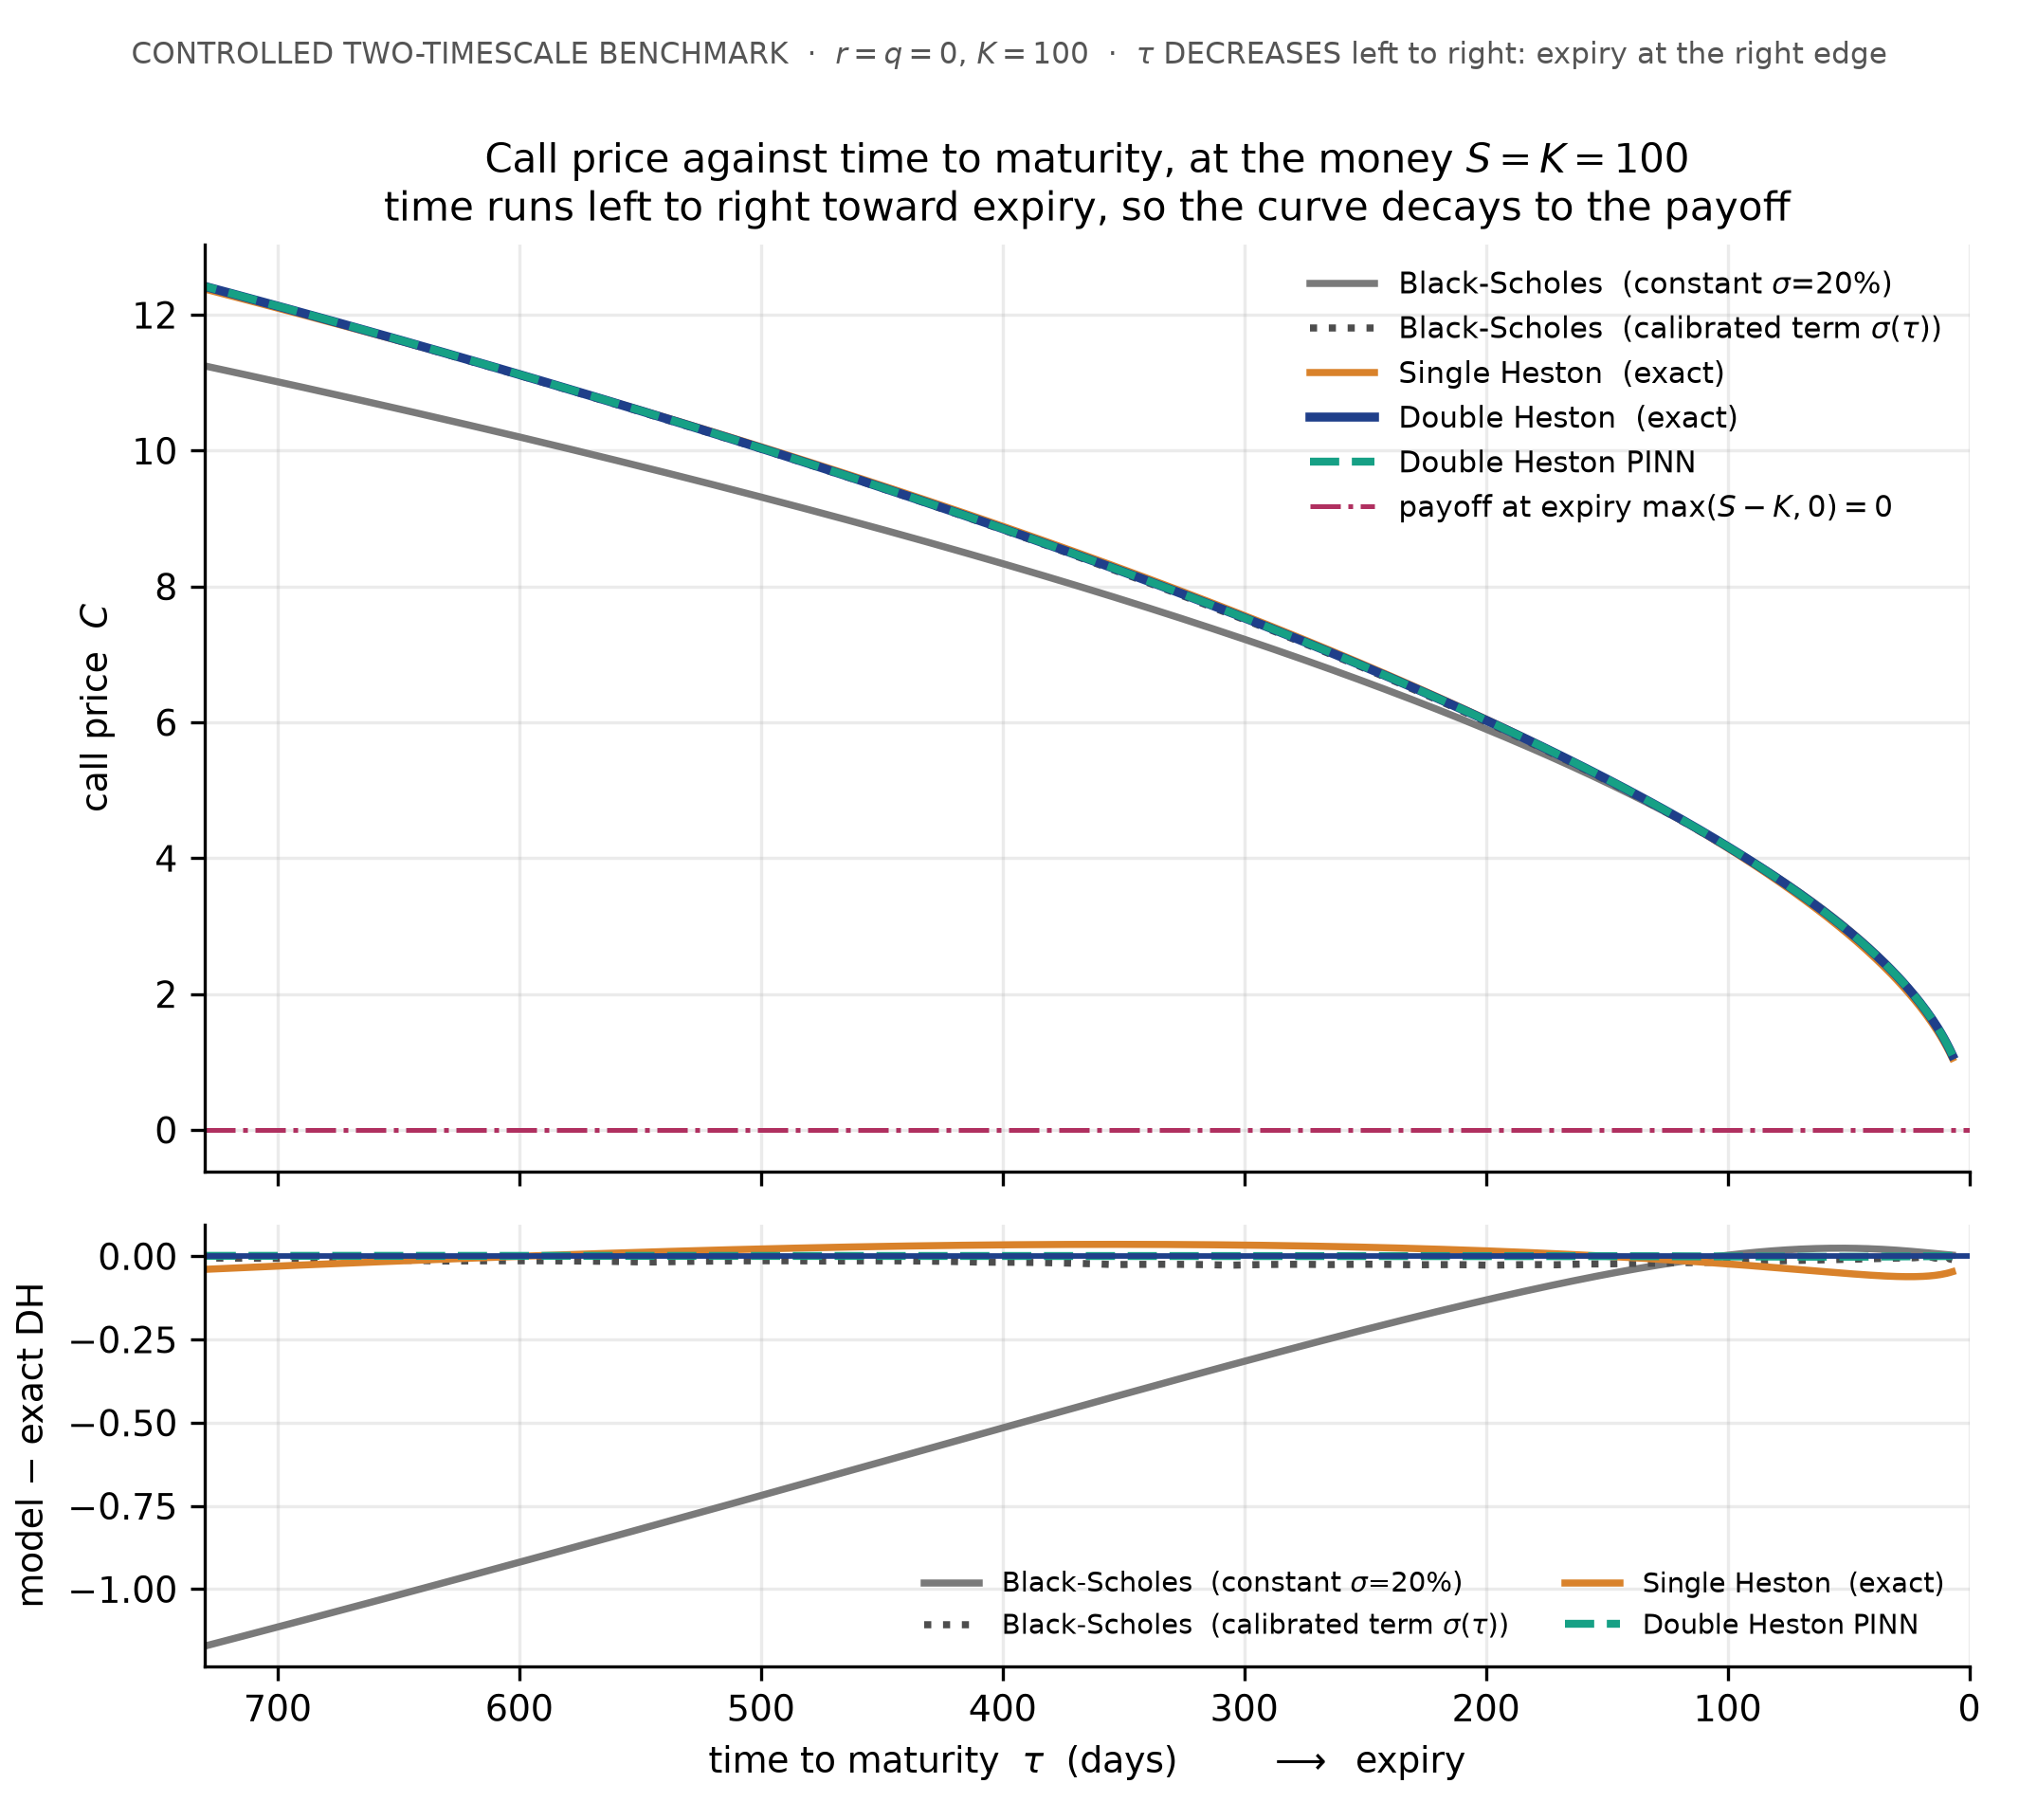
\includegraphics[width=\columnwidth]{figA2_C_vs_tau.png}
\caption{Call price against time to maturity, at the money. The maturity axis
decreases left to right, so time runs forward toward expiry and the curve
decays to the payoff.}
\label{fig:apptau}
\end{figure}

\FloatBarrier

\section{Breadth of the Market Observation}
\label{app:market}

\textbf{This appendix is outside the frozen protocol of Section~IV.} It was not
predeclared here, did not influence selection, and is not evidence for the
architectural result. It is included to show that the ceiling reported in
Section~V-C is not specific to one surface. Each result carries the disclosures
of the study that produced it.

\textbf{These are not results of this study.} The five-market Deribit
comparison in Table~\ref{tab:crypto} and the Russell~2000 comparison below are
drawn from two separate companion manuscripts by the same authors, each of
which reports its own pre-registration, calibration protocol and statistics in
full, and each of which is \emph{currently under submission elsewhere}. Their
references are withheld here only to preserve anonymous review and will be
supplied in the camera-ready version. No claim in Sections~III--VII depends on
them.

Across five cryptocurrency option markets on Deribit, with dates selected from
spot or volatility-index data before any option surface was fetched, and
significance requiring both a one-sided Wilcoxon test over clusters and a
cluster-bootstrap lower bound above zero, per-date calibrated Double Heston
beat Black--Scholes on every asset but beat Single Heston only where the market
quotes six to seven expiries per day (Table~\ref{tab:crypto}). The two markets
in which the second factor paid are the two that quote the most maturities,
which is consistent with an identifiability boundary; that mechanism is a
conjecture rather than a result, because no identifiability experiment was run
and, across only five markets, maturity coverage cannot be separated from
liquidity or length of option history. This supports the
closing recommendation: structural calibration, not network capacity, is what
moves market error.

\begin{table}[!t]
\centering
\caption{Five Deribit markets, every model calibrated per date and scored on
held-out quotes. The counts shown are the primary held-out subsets actually
scored, $5{,}214$ quotes in total; the five evaluated surfaces contain
$16{,}186$ quotes in all, the rest being used for per-date calibration.}
\label{tab:crypto}
\begin{tabular}{lrrcc}
\toprule
Asset & Held-out quotes & Expiries/day & DH $>$ SH & DH $>$ BS \\
\midrule
BTC & 2{,}223 & 7 & yes & yes \\
ETH & 1{,}509 & 6 & yes & yes \\
SOL & 658 & 4 & no & yes \\
XRP & 269 & 4 & no & yes \\
HYPE & 555 & 4 & no & yes \\
\bottomrule
\end{tabular}
\end{table}

On a Russell~2000 surface of 1,416 quotes selected in advance by a hashed
structural score, the ordering depends sharply on what is fitted. With
published parameters and only a level scale, Double Heston leads by $0.15$
volatility points out of $5.3$ ($5.301$ against $5.453$ and $5.611$). With each
model calibrated on 709 quotes and scored on the remaining 707, the gap is
large: $0.583$ against $1.893$ and $5.388$. Two disclosures apply: that
surface's model errors were known before the selection was run, so the
selection was not blind; and a domain filter applied to avoid extrapolating the
network changed the selected surface from one on which Double Heston had lost.

% =====================================================================
\begin{thebibliography}{99}

\bibitem{black1973} F.~Black and M.~Scholes, ``The pricing of options and corporate liabilities,'' \emph{Journal of Political Economy}, vol.~81, no.~3, pp.~637--654, 1973.

\bibitem{black1976} F.~Black, ``The pricing of commodity contracts,'' \emph{Journal of Financial Economics}, vol.~3, no.~1--2, pp.~167--179, 1976.

\bibitem{heston1993} S.~L. Heston, ``A closed-form solution for options with stochastic volatility with applications to bond and currency options,'' \emph{The Review of Financial Studies}, vol.~6, no.~2, pp.~327--343, 1993.

\bibitem{cjh2009} P.~Christoffersen, S.~Heston, and K.~Jacobs, ``The shape and term structure of the index option smirk: Why multifactor stochastic volatility models work so well,'' \emph{Management Science}, vol.~55, no.~12, pp.~1914--1932, 2009.

\bibitem{raissi2019} M.~Raissi, P.~Perdikaris, and G.~E. Karniadakis, ``Physics-informed neural networks: A deep learning framework for solving forward and inverse problems involving nonlinear partial differential equations,'' \emph{Journal of Computational Physics}, vol.~378, pp.~686--707, 2019.

\bibitem{karniadakis2021} G.~E. Karniadakis, I.~G. Kevrekidis, L.~Lu, P.~Perdikaris, S.~Wang, and L.~Yang, ``Physics-informed machine learning,'' \emph{Nature Reviews Physics}, vol.~3, pp.~422--440, 2021.

\bibitem{wang2021} S.~Wang, Y.~Teng, and P.~Perdikaris, ``Understanding and mitigating gradient flow pathologies in physics-informed neural networks,'' \emph{SIAM Journal on Scientific Computing}, vol.~43, no.~5, pp.~A3055--A3081, 2021.

\bibitem{wang2022} S.~Wang, X.~Yu, and P.~Perdikaris, ``When and why PINNs fail to train: A neural tangent kernel perspective,'' \emph{Journal of Computational Physics}, vol.~449, p.~110768, 2022.

\bibitem{krishnapriyan2021} A.~Krishnapriyan, A.~Gholami, S.~Zhe, R.~Kirby, and M.~W. Mahoney, ``Characterizing possible failure modes in physics-informed neural networks,'' in \emph{Advances in Neural Information Processing Systems}, vol.~34, 2021, pp.~26\,548--26\,560.

\bibitem{jagtap2020} A.~D. Jagtap, K.~Kawaguchi, and G.~E. Karniadakis, ``Adaptive activation functions accelerate convergence in deep and physics-informed neural networks,'' \emph{Journal of Computational Physics}, vol.~404, p.~109136, 2020.

\bibitem{carr1999} P.~Carr and D.~B. Madan, ``Option valuation using the fast Fourier transform,'' \emph{Journal of Computational Finance}, vol.~2, no.~4, pp.~61--73, 1999.

\bibitem{fang2008} F.~Fang and C.~W. Oosterlee, ``A novel pricing method for European options based on Fourier-cosine series expansions,'' \emph{SIAM Journal on Scientific Computing}, vol.~31, no.~2, pp.~826--848, 2008.

\bibitem{lord2010} R.~Lord and C.~Kahl, ``Complex logarithms in Heston-like models,'' \emph{Mathematical Finance}, vol.~20, no.~4, pp.~671--694, 2010.

\bibitem{cui2017} Y.~Cui, S.~del Ba\~{n}o Rollin, and G.~Germano, ``Full and fast calibration of the Heston stochastic volatility model,'' \emph{European Journal of Operational Research}, vol.~263, no.~2, pp.~625--638, 2017.

\bibitem{lagaris1998} I.~E. Lagaris, A.~Likas, and D.~I. Fotiadis, ``Artificial neural networks for solving ordinary and partial differential equations,'' \emph{IEEE Transactions on Neural Networks}, vol.~9, no.~5, pp.~987--1000, 1998.

\bibitem{sirignano2018} J.~Sirignano and K.~Spiliopoulos, ``DGM: A deep learning algorithm for solving partial differential equations,'' \emph{Journal of Computational Physics}, vol.~375, pp.~1339--1364, 2018.

\bibitem{han2018} J.~Han, A.~Jentzen, and W.~E, ``Solving high-dimensional partial differential equations using deep learning,'' \emph{Proceedings of the National Academy of Sciences}, vol.~115, no.~34, pp.~8505--8510, 2018.

\bibitem{cuomo2022} S.~Cuomo, V.~Schiano Di Cola, F.~Giampaolo, G.~Rozza, M.~Raissi, and F.~Piccialli, ``Scientific machine learning through physics-informed neural networks: Where we are and what's next,'' \emph{Journal of Scientific Computing}, vol.~92, p.~88, 2022.

\bibitem{wang2023} S.~Wang, S.~Sankaran, H.~Wang, and P.~Perdikaris, ``An expert's guide to training physics-informed neural networks,'' arXiv preprint arXiv:2308.08468, 2023.

\bibitem{wu2023} C.~Wu, M.~Zhu, Q.~Tan, Y.~Kartha, and L.~Lu, ``A comprehensive study of non-adaptive and residual-based adaptive sampling for physics-informed neural networks,'' \emph{Computer Methods in Applied Mechanics and Engineering}, vol.~403, p.~115671, 2023.

\bibitem{hutchinson1994} J.~M. Hutchinson, A.~W. Lo, and T.~Poggio, ``A nonparametric approach to pricing and hedging derivative securities via learning networks,'' \emph{The Journal of Finance}, vol.~49, no.~3, pp.~851--889, 1994.

\bibitem{ruf2020} J.~Ruf and W.~Wang, ``Neural networks for option pricing and hedging: A literature review,'' \emph{Journal of Computational Finance}, vol.~24, no.~1, pp.~1--46, 2020.

\bibitem{glau2022} K.~Glau and L.~Wunderlich, ``The deep parametric PDE method and applications to option pricing,'' \emph{Applied Mathematics and Computation}, vol.~432, p.~127355, 2022.

\bibitem{hainaut2024} D.~Hainaut and A.~Casas, ``Option pricing in the Heston model with physics inspired neural networks,'' \emph{Annals of Finance}, vol.~20, no.~3, pp.~353--376, 2024.

\bibitem{bae2024} H.-O.~Bae, S.~Kang, and M.~Lee, ``Option pricing and local volatility surface by physics-informed neural network,'' \emph{Computational Economics}, vol.~64, no.~5, pp.~3143--3159, 2024.

\bibitem{zhang2025} C.~Zhang, G.~Amici, and M.~Morandotti, ``Calibrating the Heston model with deep differential networks,'' \emph{Decisions in Economics and Finance}, 2025, doi: 10.1007/s10203-025-00558-1.

\end{thebibliography}

\end{document}
